% ---- pg-606 （书页 594） ----

\begin{mvtable}
\mvtabcap{表 6\quad $F$ 分布百分位点 $(\alpha=0.01)$}
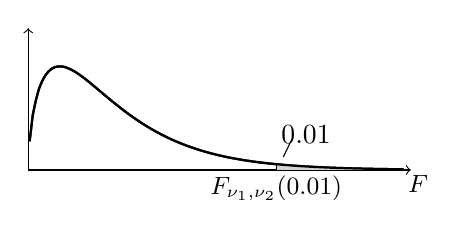
\begin{tikzpicture}[x=0.9cm,y=1.5cm]
% ---- 坐标轴 ----
\draw[->] (0,0) -- (5.4,0);
\draw[->] (0,0) -- (0,1.2);
% ---- F 分布密度曲线（近似） ----
\draw[thick,domain=0.02:5.3,samples=120]
  plot (\x,{2.6*(\x)^(0.6)*exp(-1.35*\x)});
% ---- 右侧阴影区 ----
\fill[gray!35]
  (3.5,0) -- plot[domain=3.5:5.3,samples=60]
  (\x,{2.6*(\x)^(0.6)*exp(-1.35*\x)}) -- (5.3,0) -- cycle;
\draw[thick,domain=0.02:5.3,samples=120]
  plot (\x,{2.6*(\x)^(0.6)*exp(-1.35*\x)});
% ---- 分位点竖线 ----
\draw (3.5,0) -- (3.5,{2.6*(3.5^0.6)*exp(-1.35*3.5)});
% ---- 标注 ----
\draw (3.72,0.26) -- (3.6,0.11);
\node[inner sep=1pt] at (3.92,0.30) {$0.01$};
% ---- 轴标签 ----
\node[below,inner sep=1pt,font=\small] at (3.5,-0.02) {$F_{\nu_{1},\nu_{2}}(0.01)$};
\node[below,inner sep=1pt,font=\small] at (5.5,-0.02) {$F$};
\end{tikzpicture}

{\zihao{6}
\mvfit{%
\begin{tabular}{r|*{17}{r}}
\toprule
\makecell{$\nu_{1}$\\$\nu_{2}$} & 1 & 2 & 3 & 4 & 5 & 6 & 7 & 8 & 9 & 10 & 12 & 15 & 20 & 25 & 30 & 40 & 60\\
\midrule
1 & $4\,052.0$ & $5\,000.0$ & $5\,403.0$ & $5\,625.0$ & $5\,764.0$ & $5\,859.0$ & $5\,928.0$ & $5\,981.0$ & $6\,023.0$ & $6\,056.0$ & $6\,106.0$ & $6\,157.0$ & $6\,209.0$ & $6\,240.0$ & $6\,261.0$ & $6\,287.0$ & $6\,313.0$\\
2 & 98.50 & 99.00 & 99.17 & 99.25 & 99.30 & 99.33 & 99.36 & 99.37 & 99.39 & 99.40 & 99.42 & 99.43 & 99.45 & 99.46 & 99.47 & 99.47 & 99.48\\
3 & 34.12 & 30.82 & 29.46 & 28.71 & 28.24 & 27.91 & 27.67 & 27.49 & 27.35 & 27.23 & 27.05 & 26.87 & 26.69 & 26.58 & 26.50 & 26.41 & 26.32\\
4 & 21.20 & 18.00 & 16.69 & 15.98 & 15.52 & 15.21 & 14.98 & 14.80 & 14.66 & 14.55 & 14.37 & 14.20 & 14.02 & 13.91 & 13.84 & 13.75 & 13.65\\
5 & 16.26 & 13.27 & 12.06 & 11.39 & 10.97 & 10.67 & 10.46 & 10.29 & 10.16 & 10.05 & 9.89 & 9.72 & 9.55 & 9.45 & 9.38 & 9.29 & 9.20\\
6 & 13.75 & 10.92 & 9.78 & 9.15 & 8.75 & 8.47 & 8.26 & 8.10 & 7.98 & 7.87 & 7.72 & 7.56 & 7.40 & 7.30 & 7.23 & 7.14 & 7.06\\
7 & 12.25 & 9.55 & 8.45 & 7.85 & 7.46 & 7.19 & 6.99 & 6.84 & 6.72 & 6.62 & 6.47 & 6.31 & 6.16 & 6.06 & 5.99 & 5.91 & 5.82\\
8 & 11.26 & 8.65 & 7.59 & 7.01 & 6.63 & 6.37 & 6.18 & 6.03 & 5.91 & 5.81 & 5.67 & 5.52 & 5.36 & 5.26 & 5.20 & 5.12 & 5.03\\
9 & 10.56 & 8.02 & 6.99 & 6.42 & 6.06 & 5.80 & 5.61 & 5.47 & 5.35 & 5.26 & 5.11 & 4.96 & 4.81 & 4.71 & 4.65 & 4.57 & 4.48\\
10 & 10.04 & 7.56 & 6.55 & 5.99 & 5.64 & 5.39 & 5.20 & 5.06 & 4.94 & 4.85 & 4.71 & 4.56 & 4.41 & 4.31 & 4.25 & 4.17 & 4.08\\
11 & 9.65 & 7.21 & 6.22 & 5.67 & 5.32 & 5.07 & 4.89 & 4.74 & 4.63 & 4.54 & 4.40 & 4.25 & 4.10 & 4.01 & 3.94 & 3.86 & 3.78\\
12 & 9.33 & 6.93 & 5.95 & 5.41 & 5.06 & 4.82 & 4.64 & 4.50 & 4.39 & 4.30 & 4.16 & 4.01 & 3.86 & 3.76 & 3.70 & 3.62 & 3.54\\
13 & 9.07 & 6.70 & 5.74 & 5.21 & 4.86 & 4.62 & 4.44 & 4.30 & 4.19 & 4.10 & 3.96 & 3.82 & 3.66 & 3.57 & 3.51 & 3.43 & 3.34\\
14 & 8.86 & 6.51 & 5.56 & 5.04 & 4.69 & 4.46 & 4.28 & 4.14 & 4.03 & 3.94 & 3.80 & 3.66 & 3.51 & 3.41 & 3.35 & 3.27 & 3.18\\
15 & 8.68 & 6.36 & 5.42 & 4.89 & 4.56 & 4.32 & 4.14 & 4.00 & 3.89 & 3.80 & 3.67 & 3.52 & 3.37 & 3.28 & 3.21 & 3.13 & 3.05\\
\bottomrule
\end{tabular}
}}
\end{mvtable}
